\documentclass[11pt]{article}

% Change "review" to "final" to generate the final (sometimes called camera-ready) version.
% Change to "preprint" to generate a non-anonymous version with page numbers.
\usepackage[preprint]{acl}

% Standard package includes
\usepackage{times}
\usepackage{latexsym}
\usepackage{caption}
% For proper rendering and hyphenation of words containing Latin characters (including in bib files)
\usepackage[T1]{fontenc}
% For Vietnamese characters
% \usepackage[T5]{fontenc}
% See https://www.latex-project.org/help/documentation/encguide.pdf for other character sets

% This assumes your files are encoded as UTF8
\usepackage[utf8]{inputenc}

% This is not strictly necessary, and may be commented out,
% but it will improve the layout of the manuscript,
% and will typically save some space.
\usepackage{microtype}
\usepackage{booktabs} 
\usepackage{multirow} 
% This is also not strictly necessary, and may be commented out.
% However, it will improve the aesthetics of text in
% the typewriter font.
\usepackage{inconsolata}

%Including images in your LaTeX document requires adding
%additional package(s)
\usepackage{graphicx}
\usepackage{amsmath}
\usepackage{amsfonts}
\usepackage{url}
\usepackage[table]{xcolor}

% Define colors for top-3 highlighting
\definecolor{gold}{RGB}{255, 215, 0}
\definecolor{silver}{RGB}{192, 192, 192}
\definecolor{bronze}{RGB}{205, 127, 50}

% If the title and author information does not fit in the area allocated, uncomment the following
%
%\setlength\titlebox{<dim>}
%
% and set <dim> to something 5cm or larger.

\title{Discriminative vs. Generative Approaches for Visual Word Sense Disambiguation: An Empirical Study}

% Author information can be set in various styles:
% For several authors from the same institution:
% \author{Rui Zhou \and Jiawei Pei \and Author n \\
%         Address line \\ ... \\ Address line}
% if the names do not fit well on one line use
%         Author 1 \\ {\bf Author 2} \\ ... \\ {\bf Author n} \\
% For authors from different institutions:
% \author{Author 1 \\ Address line \\  ... \\ Address line
%         \And  ... \And
%         Author n \\ Address line \\ ... \\ Address line}
% To start a separate ``row'' of authors use \AND, as in
% \author{Author 1 \\ Address line \\  ... \\ Address line
%         \AND
%         Author 2 \\ Address line \\ ... \\ Address line \And
%         Author 3 \\ Address line \\ ... \\ Address line}

\author{Rui Zhou \\
  University of Zurich\\
  % Affiliation / Address line 2 \\
  % Affiliation / Address line 3 \\
  \texttt{rui.zhou2@uzh.ch} \\\And
  Jiawei Pei \\
  University of Zurich\\
  % Affiliation / Address line 2 \\
  % Affiliation / Address line 3 \\
  \texttt{jiawei.pei@uzh.ch} \\\And
  Nilaksan Selliah \\
  University of Zurich\\
  % Affiliation / Address line 2 \\
  % Affiliation / Address line 3 \\
  \texttt{nilaksan.selliah@uzh.ch} \\} 

\begin{document}
\maketitle
\begin{abstract}
Visual Word Sense Disambiguation (VWSD) requires selecting the correct image for an ambiguous word given minimal context---a task where even large vision-language models struggle. We systematically compare discriminative embedding methods versus generative reasoning on the SemEval-2023 Task 1 benchmark, evaluating SigLIP2 against Qwen3-VL across five inference strategies. Our key findings reveal that: (1) \textbf{training objectives matter more than scale}---SigLIP2 (1B params) outperforms Qwen3-VL embeddings (8B params) by 63 points, as retrieval-optimized representations fundamentally differ from generation-optimized ones; (2) \textbf{generation bridges representation gaps}---while VLM embeddings fail catastrophically (9.07\%), explicit reasoning via Chain-of-Thought reaches 65.44\%, though still trailing discriminative methods; (3) \textbf{knowledge augmentation often backfires}---injecting sense definitions hurts both paradigms, revealing distribution mismatch between structured definitions and natural training captions; (4) \textbf{cascade reranking achieves synergistic gains}---combining SigLIP2 retrieval with VLM reranking yields 77.32\% Hit@1, exploiting complementary failure modes. For fine-tuning, naive LoRA causes negative transfer ($-$0.64\%), but VLM-generated text augmentation recovers gains (+1.95\%). Code: \url{https://github.com/JaveyBae/Essentials-for-NLP}.
\end{abstract}

\section{Introduction}

Consider the phrase ``bank deposit'': should an image retrieval system return a riverbank or a financial institution? Humans resolve such ambiguities effortlessly, but this task---Visual Word Sense Disambiguation (VWSD)---remains challenging for modern vision-language models. While textual Word Sense Disambiguation has been extensively studied \cite{bevilacqua-etal-2021-recent}, its visual counterpart requires reasoning across both modalities with minimal context.

The SemEval-2023 Task 1 \cite{raganato2023semeval} formalized VWSD as a benchmark with three core challenges: (1) \textbf{sparse context}---typically just one or two words accompany the target; (2) \textbf{fine-grained distractors}---candidates include both alternative word senses and visually similar images from the same domain; and (3) \textbf{zero-shot transfer}---systems must generalize without task-specific training. Despite 96 submissions, zero-shot CLIP achieved only 37.20\% accuracy, underscoring the difficulty.

Two paradigms have emerged for multimodal understanding: \textit{discriminative} dual-encoders optimized for retrieval, and \textit{generative} vision-language models (VLMs) capable of reasoning. Which approach better handles VWSD's unique challenges? This question motivates our study.

We systematically compare \textbf{SigLIP2} \cite{zhai2023siglip}, a dual-encoder with sigmoid loss for better-calibrated ranking, against \textbf{Qwen3-VL} \cite{yang2025qwen3}, an 8B-parameter VLM evaluated across five inference strategies. We also evaluate \textbf{CLIP} variants \cite{radford2021clip} as baselines, \textbf{cascade reranking} combining fast retrieval with focused VLM reasoning, and \textbf{LoRA fine-tuning} with VLM-generated text augmentation.

\noindent\textbf{Key Contributions:}
\begin{enumerate}
    \item We establish that \textbf{pre-training objectives matter more than scale}: SigLIP2 outperforms Qwen3-VL embeddings by 63 points despite being 8$\times$ smaller.
    \item We show that \textbf{generation bridges representation gaps}: CoT prompting partially recovers VLM performance, but \textbf{injected knowledge often hurts}---sense definitions degrade both paradigms.
    \item We demonstrate that \textbf{cascade reranking exploits complementary failures}: combining SigLIP2 with VLM reranking yields 77.32\% Hit@1.
    \item We provide \textbf{practical fine-tuning guidance}: naive LoRA causes negative transfer, but VLM-generated text augmentation preserves pre-trained distributions.
\end{enumerate}

The remainder of this paper is structured as follows: Section~\ref{sec:related} surveys prior work on visual disambiguation and multimodal retrieval; Section~\ref{sec:method} details our discriminative and generative approaches; Section~\ref{sec:experiments} presents experimental setup, results, and comparative analysis; Section~\ref{sec:limitations} discusses limitations; and Section~\ref{sec:conclusion} concludes with future directions.

\section{Related Work}
\label{sec:related}

\subsection{Visual Word Sense Disambiguation}

Visual Word Sense Disambiguation was formalized as SemEval-2023 Task 1 by \citet{raganato2023semeval}. The task received 96 submissions from 56 teams across three languages, revealing the complexity of multimodal disambiguation. The zero-shot CLIP baseline achieved only 37.20\% Hit@1, substantially lower than traditional textual WSD benchmarks, emphasizing the need for context-aware cross-modal reasoning.

\textbf{Knowledge Retrieval and Ensemble Approaches.} The top-performing systems employed sophisticated retrieval-augmented pipelines. \citet{zhang2023srcb} (SRCB, 1st place in English with 84.02\% Hit@1) leveraged external knowledge bases including WordNet, BabelNet, Wikipedia, and vocabulary.com to construct comprehensive sense inventories. They retrieved definitions and synonyms for the target word, then collected relevant images from the LAION-5B dataset using CLIP-based retrieval. A SimCSE-based biencoder selected the most suitable definition, which was then matched against candidate images using a large CLIP model trained on LAION-2B. Notably, SRCB translated senses from English for Italian and Farsi, achieving strong cross-lingual transfer.

\textbf{Fine-Grained Contrastive Learning.} \citet{yang2023fcll} (FCLL, 1st place overall with 72.56\% average Hit@1) proposed a Fine-grained Contrastive Language-Image Learning framework that learns hierarchical word-sense-image relationships. Their approach introduced a ``sense auto-complementing'' module to enrich minimal context by establishing relationships between concepts and sentences. They constructed a multilingual multimodal knowledge base for ambiguous words, enabling robust cross-lingual performance. This method demonstrated the importance of explicitly modeling sense-level distinctions rather than treating disambiguation as simple image classification.

\textbf{Hybrid Knowledge-Based Systems.} \citet{dadas2023opi} (3rd place overall, 1st in Farsi with 64.0\% Hit@1) combined multimodal embeddings with knowledge-based approaches. Their system integrated CLIP embeddings with additional information retrieved from Wikipedia and lexical databases, using a learning-to-rank (LTR) model to combine outputs from multiple modules. This hybrid approach demonstrates that structured knowledge can complement learned representations, particularly for languages with limited training data.

Other notable approaches include ensemble methods combining multiple CLIP variants with translation models \cite{patil2023rahul}, text-to-image generation for synthetic data augmentation \cite{li2023augmenters}, and prompt augmentation strategies \cite{ghahroodi-etal-2023-sut}. However, nearly all top systems relied on zero-shot or few-shot approaches due to the limited size of training data (12,869 instances), highlighting the importance of strong pre-training for this task.

\subsection{Vision-Language Pre-Training}

\textbf{Contrastive Dual-Encoders.} CLIP \cite{radford2021clip} pioneered large-scale contrastive vision-language pre-training, training separate image and text encoders to align embeddings in a shared space using InfoNCE loss. However, CLIP's batch-based contrastive objective can lead to suboptimal calibration for retrieval tasks. SigLIP \cite{zhai2023siglip} addresses this by replacing InfoNCE with sigmoid loss, which operates on image-text pairs independently rather than requiring large batches. This pairwise classification approach improves retrieval performance and enables more efficient training. Our work leverages SigLIP2, the second generation of this architecture, demonstrating its effectiveness for fine-grained disambiguation.

\textbf{Generative Vision-Language Models.} Recent advances in autoregressive vision-language models have enabled explicit reasoning over visual content. Models like GPT-4V \cite{openai2023gpt4v}, Qwen-VL \cite{bai2023qwen}, and LLaVA \cite{liu2023llava} unify visual perception with language generation, allowing for interpretable decision-making through Chain-of-Thought prompting \cite{wei2022chain}. While these models excel at open-ended visual question answering, their effectiveness for structured ranking tasks like VWSD remains underexplored. Our work investigates whether generative reasoning can match or exceed discriminative retrieval for disambiguation.

\textbf{Multimodal Disambiguation Tasks.} Beyond VWSD, related work includes image-text retrieval \cite{li2020oscar}, visual grounding \cite{kazemzadeh2014referit}, and multimodal lexical semantics \cite{calabrese2020evilbert}. BabelPic \cite{calabrese2020babelpic} provided a multimodal dataset for non-concrete concepts, demonstrating the challenges of representing abstract meanings visually. Our work extends this line of research by focusing on the specific challenge of sense-level disambiguation under minimal context, which requires both fine-grained semantic understanding and robust cross-modal alignment.

\section{Methodology}
\label{sec:method}

We investigate two fundamental paradigms for Visual Word Sense Disambiguation: (1) \textit{discriminative} embedding-based retrieval, and (2) \textit{generative} vision-language reasoning. We also explore knowledge augmentation strategies and hybrid architectures that combine both paradigms. All methods rank 10 candidate images given a target word and minimal context.

\subsection{Task Formalization}

Given an ambiguous target word $w$, a textual context $c$ containing $w$, and a set of $n=10$ candidate images $\mathcal{I} = \{I_1, I_2, \ldots, I_n\}$, the task is to produce a ranking $\pi$ such that the gold image $I^*$ appears as high as possible. Each method computes a relevance score $s_i$ for each image $I_i$, yielding the final ranking $\pi = \text{argsort}(\{s_1, \ldots, s_n\})$.

\subsection{Discriminative Retrieval}

Discriminative methods encode text and images into a shared embedding space, ranking by similarity scores.

\subsubsection{SigLIP2}

SigLIP2 \cite{zhai2023siglip} employs a dual-encoder architecture with separate vision and text transformers. Unlike CLIP's \cite{radford2021clip} InfoNCE loss, SigLIP2 uses sigmoid loss for pairwise classification:
\begin{equation}
\mathcal{L} = -\sum_{i,j} \left[ z_{ij} \log \sigma(s_{ij}) + (1-z_{ij}) \log (1 - \sigma(s_{ij})) \right]
\end{equation}
where $s_{ij} = f_v(I_i)^\top f_t(T_j)$ is the similarity score, $z_{ij} \in \{0, 1\}$ indicates pairing, and $\sigma$ is the sigmoid function. This formulation provides better-calibrated scores for ranking tasks.

For inference, we construct a query $q$ using the format ``this is a photo of a $w$. $c$'' and encode it alongside all candidate images, ranking by $s_i = \sigma(f_t(q)^\top f_v(I_i))$.

\subsubsection{VLM Embedding Extraction}

As an alternative discriminative approach, we extract embeddings from Qwen3-VL \cite{yang2025qwen3} without generation. Text queries are encoded through the language model with mean pooling over hidden states; images are processed similarly. Ranking uses cosine similarity: $s_i = \text{cosine}(f_{\text{text}}(q), f_{\text{image}}(I_i))$. This tests whether VLM representations transfer to retrieval despite being optimized for generation.

\subsection{Generative Reasoning}

Generative methods leverage vision-language models to produce explicit reasoning about image-text matches.

\subsubsection{Direct Matching}

Qwen3-VL \cite{yang2025qwen3} is an autoregressive VLM that integrates a vision encoder with a causal language model. For each candidate image, the model rates relevance on a 0--10 scale given the target word and context. Scores are normalized for ranking.

\subsubsection{Chain-of-Thought (CoT)}

We extend direct matching with step-by-step reasoning \cite{wei2022chain}: (1) interpret the word's meaning in context, (2) describe what the image shows, (3) assess the match. The model outputs brief reasoning followed by a numeric rating.

\subsubsection{Caption-to-Text Pipeline}

Rather than having the VLM directly rate images, we test whether generating captions and computing text-only similarity is effective. Qwen3-VL generates a description for each candidate image, and Sentence-BERT \cite{reimers2019sentence} computes cosine similarity between the query and each caption. This decouples visual understanding from similarity computation.

\subsection{Knowledge Augmentation}

We investigate whether enriching queries with external knowledge improves disambiguation.

\subsubsection{Sense Definition Enrichment}

We employ a two-stage pipeline using language models to generate visual sense definitions---short, concrete descriptions of what would appear in an image for the intended meaning. For example, ``river bank'' yields \textit{``Sloped land beside a river or stream.''} These definitions can be injected into queries for both discriminative and generative methods.

For discriminative retrieval (SigLIP2), we test three query variants: (1) appending definitions to the original query, (2) replacing context with definitions, and (3) using definitions only. For generative methods (Qwen3-VL), definitions are provided as ``visual clues'' to guide image rating.

\subsubsection{Text-to-Image Synthesis}

As an alternative knowledge augmentation strategy, we generate synthetic images representing the intended word sense using text-to-image diffusion models. Given a query, we first expand it into semantically enriched variants using an LLM, then generate a synthetic image $\hat{v}$ via an API-based diffusion model.

Retrieval then operates entirely in the visual embedding space:
\[
    s(q, v_i) = \cos\left(f(\hat{v}), f(v_i)\right)
\]
where $f(\cdot)$ is a vision encoder. This approach reduces cross-modal mismatch by comparing images directly, using the generated image as a visual proxy for the textual query.

\subsection{Cascade Reranking}

Motivated by the complementary strengths of discriminative retrieval (fast, well-calibrated) and generative reasoning (interpretable, context-aware), we propose a two-stage cascade pipeline:

\textbf{Stage 1: Fast Retrieval.} SigLIP2 ranks all 10 candidate images using embedding similarity, efficiently filtering obvious mismatches.

\textbf{Stage 2: Focused Reranking.} Qwen3-VL with Chain-of-Thought reasoning reranks only the top-$K$ candidates from Stage 1, concentrating computational resources on cases where fine-grained disambiguation is needed.

The final ranking concatenates the VLM-reranked top-$K$ with the remaining SigLIP2-ranked candidates: $\pi_{\text{final}} = [\pi_{\text{VLM}}^{1:K}] \oplus [\pi_{\text{SigLIP2}}^{K+1:10}]$.

\subsection{Parameter-Efficient Fine-Tuning}

To adapt discriminative models for VWSD while preserving their general visual-linguistic capabilities, we employ Low-Rank Adaptation (LoRA) \cite{hu2022lora}. LoRA introduces trainable rank-decomposition matrices into transformer layers while keeping pre-trained weights frozen:
\begin{equation}
h = W_0 x + \frac{\alpha}{r} BA x
\end{equation}
where $W_0$ is the frozen pre-trained weight, $B \in \mathbb{R}^{d \times r}$ and $A \in \mathbb{R}^{r \times d}$ are trainable low-rank matrices, $r$ is the rank, and $\alpha$ is a scaling factor.

We apply LoRA to attention projection layers (\texttt{q\_proj}, \texttt{k\_proj}, \texttt{v\_proj}, \texttt{out\_proj}) while freezing the vision encoder entirely. Training uses SigLIP-style sigmoid contrastive loss:
\begin{equation}
\mathcal{L} = -\log \sigma(s^+) - \sum_{j=1}^{N} \log \sigma(-s_j^-)
\end{equation}
where $s^+ = f_t(q)^\top f_v(I^+)$ is the positive similarity and $s_j^-$ are similarities with $N$ hard negatives (other candidate images for the same word). We disable in-batch negatives to avoid false negative issues when different instances share semantically similar correct images.

\subsection{VLM-Based Text Augmentation}

To combat overfitting on limited training data, we augment text queries using VLMs. We generate three augmentation types offline:

\textbf{Captions}: Natural descriptions of gold images generated by a VLM, providing image-grounded alternatives to the minimal original context.

\textbf{Definitions}: Visual sense definitions that describe what would appear in an image for the intended meaning, offering semantically precise but stylistically different queries.

\textbf{Paraphrases}: Multiple rephrased variants of the context phrase that preserve the target word, increasing lexical diversity.

During training, original queries are replaced with augmented versions with probability $p_{\text{aug}}$, with uniform random selection among available augmentation types.

\section{Experiments}
\label{sec:experiments}

\subsection{Dataset and Evaluation Metrics}

We use the SemEval-2023 Task 1 English test set, comprising 463 instances with manually annotated gold images. Each instance includes a target word, minimal context (1--2 words), and 10 candidate images. The dataset emphasizes challenging disambiguation scenarios: at least one candidate represents an incorrect sense of the target word, and other distractors are sampled from the same semantic domain (e.g., different animals for ``crane habitat'').

We evaluate using three standard ranking metrics:

\textbf{Hit@1 (Accuracy)} measures the proportion of queries where the gold image is ranked first:
\begin{equation}
\text{Hit@1} = \frac{1}{|\mathcal{Q}|} \sum_{i=1}^{|\mathcal{Q}|} \mathbb{1}[\text{rank}_i = 1]
\end{equation}
where $\text{rank}_i$ is the position of the gold image for query $i$.

\textbf{Mean Reciprocal Rank (MRR)} emphasizes the rank of the first correct result:
\begin{equation}
\text{MRR} = \frac{1}{|\mathcal{Q}|} \sum_{i=1}^{|\mathcal{Q}|} \frac{1}{\text{rank}_i}
\end{equation}

\textbf{Normalized Discounted Cumulative Gain (NDCG@k)} accounts for graded relevance and position:
\begin{equation}
\text{NDCG@k} = \frac{\sum_{i=1}^{k} \frac{2^{\text{rel}_i} - 1}{\log_2(i+1)}}{\sum_{i=1}^{|\text{rel}|} \frac{2^{\text{rel}_i} - 1}{\log_2(i+1)}}
\end{equation}

Hit@1 and MRR are the official metrics for VWSD; we additionally report NDCG@5 and NDCG@10 to assess ranking quality at different depths.

\subsection{Implementation Details}

All experiments use Hugging Face Transformers on NVIDIA GPUs. We describe implementations for each approach category below.

\textbf{Discriminative Models.} For \textbf{CLIP}, we use \texttt{openai/clip-vit-base-patch32} with the prompt template ``This is [mask]. [target\_phrase]''. For \textbf{SigLIP2}, we use the \texttt{so400m-patch14-384} variant (1B parameters, 384px resolution) with Flash Attention 2, encoding one query and 10 images per forward pass (2--4 GB VRAM).

\textbf{Generative Models.} \textbf{Qwen3-VL 8B} uses bfloat16 precision with temperature 0.0 for deterministic generation (16--24 GB VRAM). \textbf{Sense definitions} are generated using Qwen3-8B text models with few-shot prompting and cached to avoid regeneration. \textbf{Text-to-image synthesis} uses Gemini's Imagen API. For cascade reranking, we use $K=5$ candidates.

\textbf{Fine-Tuning.} We apply LoRA to both CLIP (\texttt{laion/CLIP-ViT-L-14}) and SigLIP2 (\texttt{google/siglip2-base-patch16-512}), using rank $r=16$, scaling factor $\alpha=32$, and dropout 0.1. Training employs AdamW with learning rate $5 \times 10^{-6}$ (reduced from an initial $2 \times 10^{-5}$ to prevent catastrophic forgetting), batch size 8, and gradient accumulation over 4 steps (effective batch size 32). We train for up to 10 epochs with bfloat16 mixed precision, 10\% linear warmup, and cosine learning rate schedule. Early stopping with patience 2 halts training when validation MRR stops improving. The configuration adds only $\sim$2M trainable parameters to the $\sim$878M frozen base model.

\textbf{Text Augmentation.} We generate augmentations for 12,840 training instances (99.8\% coverage) using Qwen3-VL-8B for captions (natural image descriptions, max 150 tokens) and Qwen3-8B for definitions and paraphrases (3 variants per instance). This yields approximately 51,000 augmented text variants. During training, original queries are replaced with augmented versions with probability $p_{\text{aug}}=0.5$.

\subsection{Training Dynamics}

Fine-tuning on the limited VWSD training data (12,869 instances) presents significant overfitting challenges. Our initial experiments with learning rate $2 \times 10^{-5}$ showed rapid performance degradation after just 1--2 epochs, with validation MRR dropping while training loss continued to decrease---a classic overfitting signature.

We implemented several mitigation strategies: (1) reduced learning rate ($5 \times 10^{-6}$) to slow catastrophic forgetting; (2) early stopping based on validation MRR with patience 2; (3) text augmentation (50\% replacement probability) to increase training diversity; and (4) cosine annealing with 10\% linear warmup.

\begin{figure}[t]
    \centering
    \begin{minipage}{0.48\columnwidth}
        \centering
        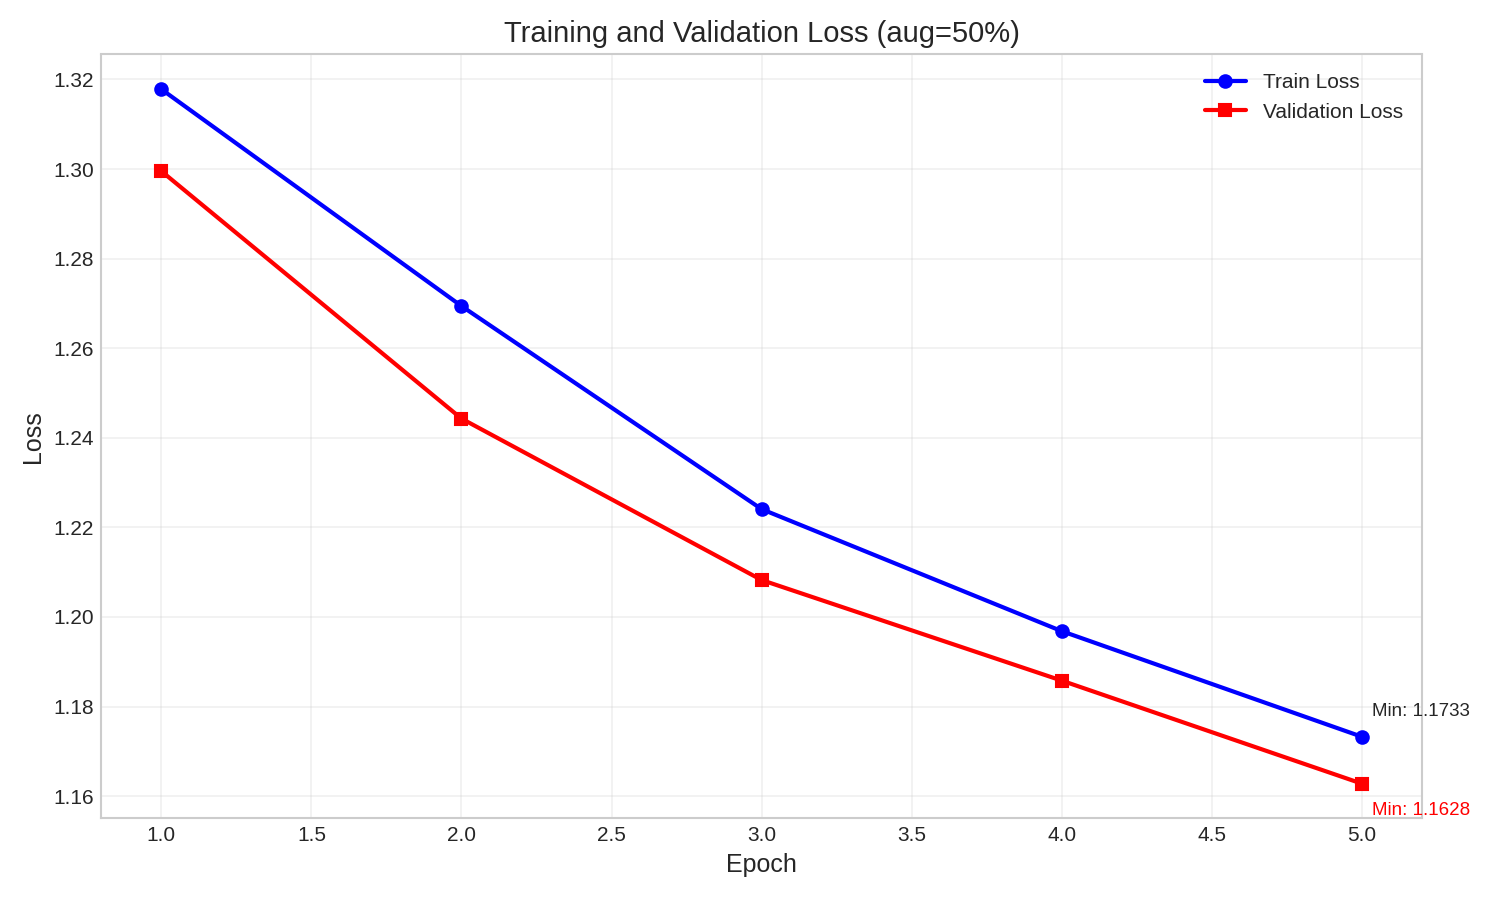
\includegraphics[width=\textwidth]{images/loss_curves.png}
        \caption*{(a) Loss Curves}
    \end{minipage}
    \hfill
    \begin{minipage}{0.48\columnwidth}
        \centering
        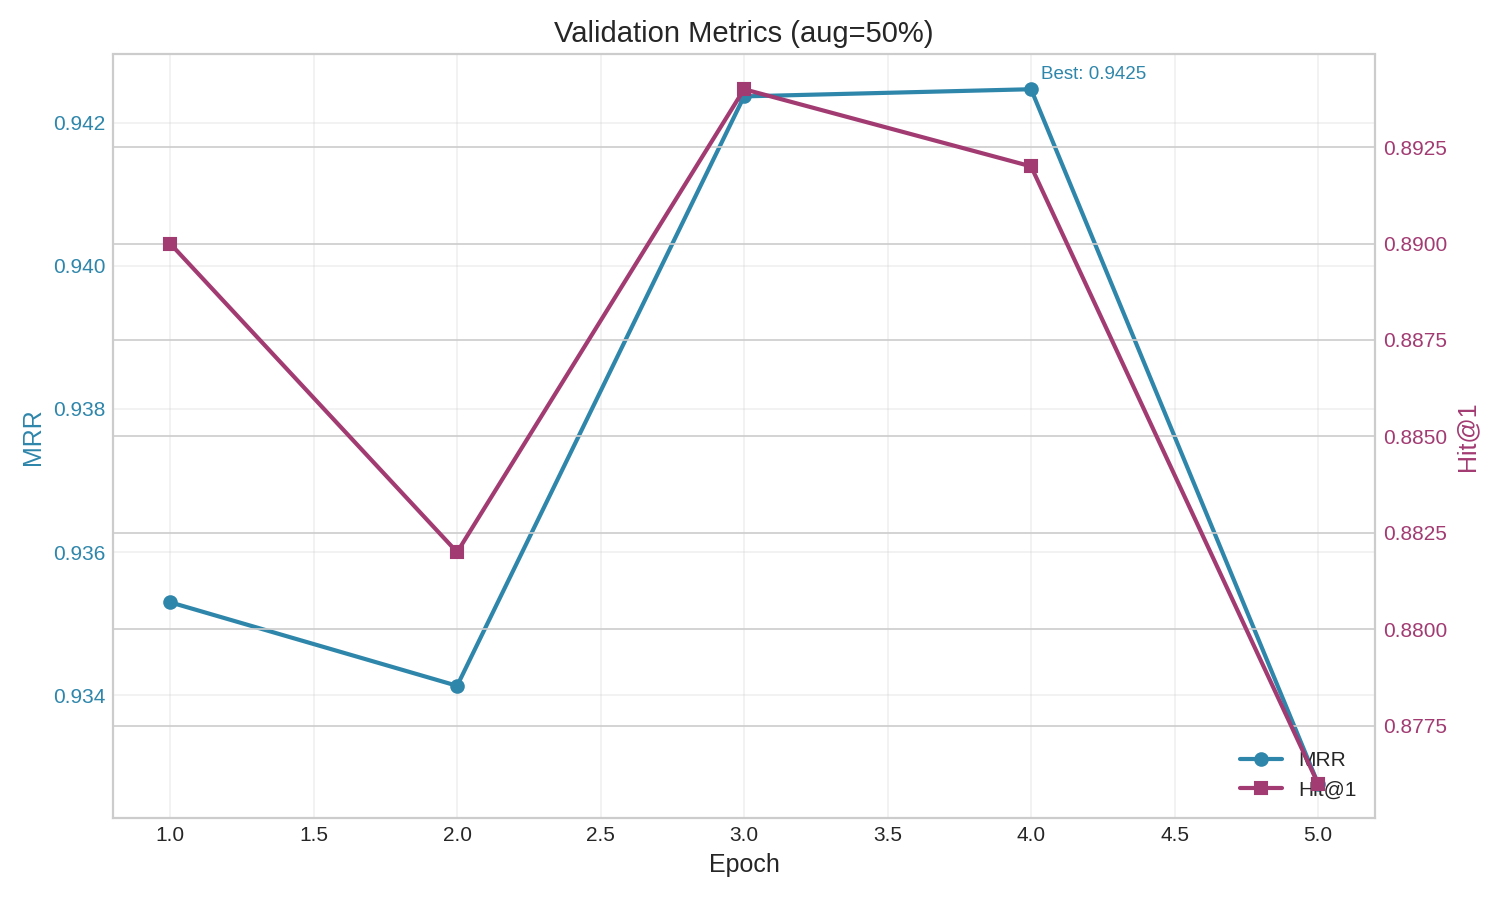
\includegraphics[width=\textwidth]{images/metrics_curves.png}
        \caption*{(b) Validation Metrics}
    \end{minipage}
    \caption{Training dynamics for SigLIP2 LoRA fine-tuning \textbf{with} 50\% text augmentation. (a) Loss curves exhibit parallel descent for training and validation sets without divergence, indicating effective regularization. (b) Validation MRR peaks at 0.9424 (epoch 3--4) before declining to 0.9328 at epoch 5, triggering early stopping. Test Hit@1 reaches 69.98\%, a 1.95-point improvement over the zero-shot baseline.}
    \label{fig:training_curves}
\end{figure}

Figure~\ref{fig:training_curves} shows the training dynamics with our final configuration (with text augmentation). The training and validation losses decrease in parallel without diverging, indicating healthy generalization. Early stopping triggered at epoch 5 (of 10 maximum) when validation MRR failed to improve for 2 consecutive epochs. The validation metrics reveal important patterns: MRR initially fluctuates (0.935 at epoch 1, 0.934 at epoch 2) before reaching its peak at epoch 3--4 (0.9424), then declining to 0.9328 at epoch 5. This non-monotonic behavior underscores the importance of early stopping.

\begin{figure}[t]
    \centering
    \begin{minipage}{0.48\columnwidth}
        \centering
        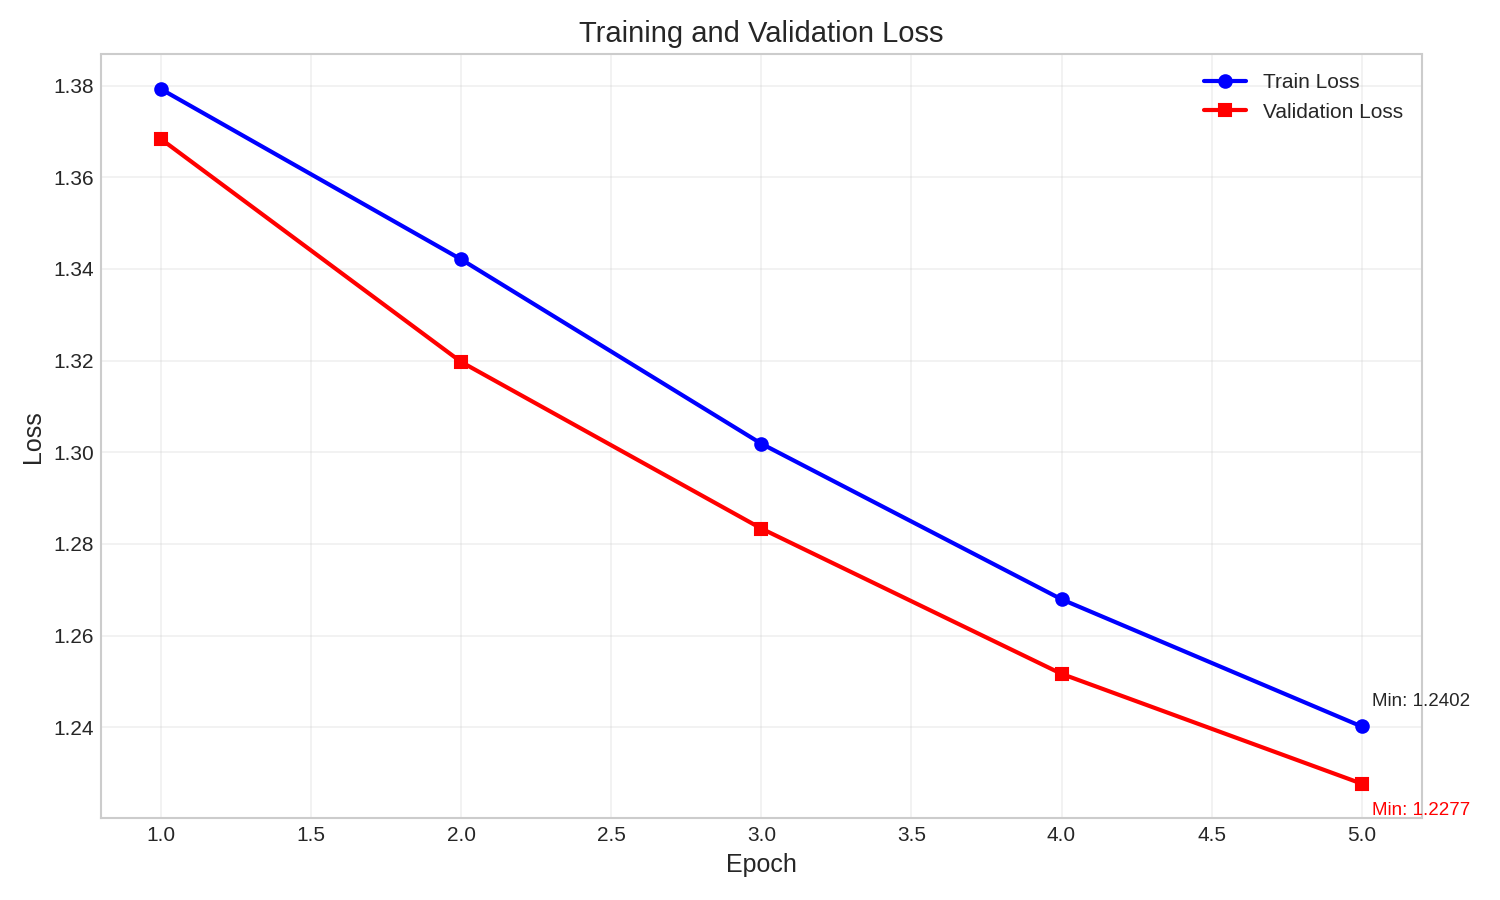
\includegraphics[width=\textwidth]{images/loss_curves_no_aug.png}
        \caption*{(a) Without Augmentation}
    \end{minipage}
    \hfill
    \begin{minipage}{0.48\columnwidth}
        \centering
        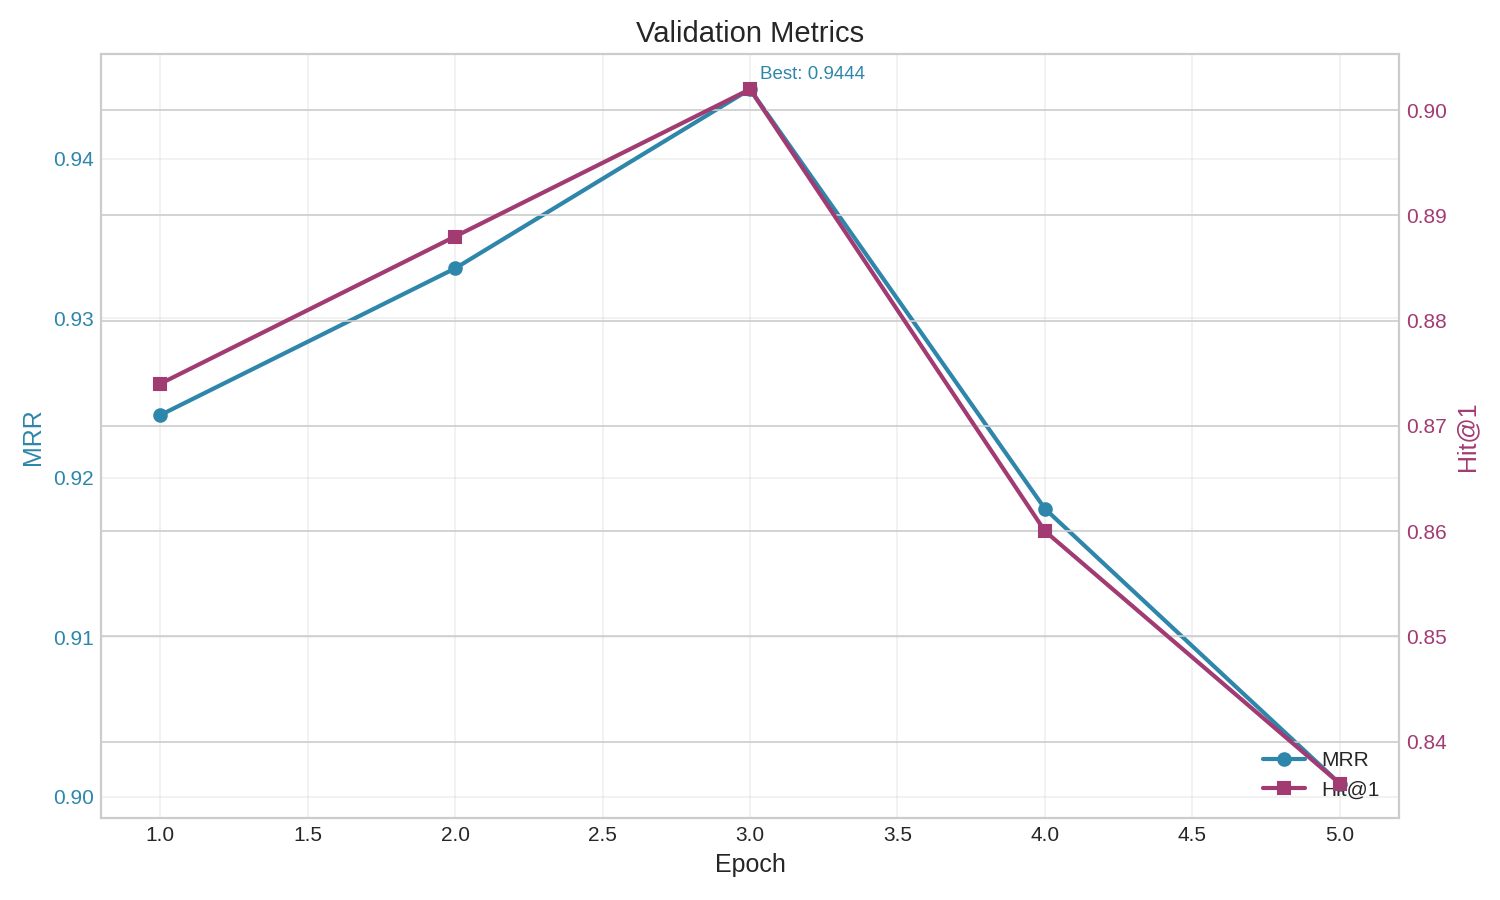
\includegraphics[width=\textwidth]{images/metrics_curves_no_aug.png}
        \caption*{(b) Validation Metrics (No Aug)}
    \end{minipage}
    \caption{Training dynamics for SigLIP2 LoRA fine-tuning \textbf{without} text augmentation. (a) Loss curves show apparent convergence with decreasing training and validation loss. (b) Validation MRR peaks at 0.9444 (epoch 3) before declining sharply to 0.9008 by epoch 5. Despite ostensibly healthy training dynamics, test Hit@1 drops to 67.39\%---0.64 points \textit{below} the 68.03\% zero-shot baseline, demonstrating negative transfer.}
    \label{fig:training_comparison}
\end{figure}

\subsection{Main Results}

Table~\ref{tab:results} presents our main results on the English test set (463 instances). We organize methods into four categories and analyze performance across Hit@1, MRR, and NDCG@10.

\begin{table}[!ht]
\centering
\small
\resizebox{\columnwidth}{!}{%
\begin{tabular}{l|ccc}
\toprule
\textbf{Method} & \textbf{Hit@1} & \textbf{MRR} & \textbf{NDCG} \\
\midrule
\multicolumn{4}{l}{\textit{SemEval-2023 Winners (with external knowledge)}} \\
\midrule
SRCB \cite{zhang2023srcb} & \cellcolor{gold}84.02 & \cellcolor{gold}89.56 & -- \\
FCLL \cite{yang2023fcll} & \cellcolor{silver}80.13 & \cellcolor{silver}87.42 & -- \\
OPI \cite{dadas2023opi} & \cellcolor{bronze}77.97 & \cellcolor{bronze}85.88 & -- \\
\midrule
\multicolumn{4}{l}{\textit{CLIP (Zero-Shot)}} \\
\midrule
ViT-B/32 & 61.34 & 74.66 & 80.83 \\
ViT-L/14 & 61.98 & 75.70 & 81.98 \\
ViT-H/14 & 63.28 & 76.99 & 76.16 \\
ViT-G/14 & 65.65 & 78.56 & 81.94 \\
\midrule
\multicolumn{4}{l}{\textit{CLIP + Augmentation (Zero-Shot)}} \\
\midrule
ViT-L/14 + Text2Image & 65.23 & 76.39 & 82.86 \\
ViT-L/14 + Text Aug & 73.43 & 83.29 & \cellcolor{bronze}87.65 \\
\midrule
\multicolumn{4}{l}{\textit{SigLIP2 (Zero-Shot)}} \\
\midrule
Base (patch16-512) & 68.03 & 79.81 & 84.77 \\
so400m (patch14-384) & 72.79 & 82.76 & 87.00 \\
\quad + def (append) & 72.57 & 82.05 & 86.42 \\
\quad + def (replace) & 69.11 & 79.58 & 84.53 \\
\quad + def (only) & 61.34 & 74.46 & 80.67 \\
\midrule
\multicolumn{4}{l}{\textit{Qwen3-VL 8B (Generative)}} \\
\midrule
Embedding & 9.07 & 29.31 & 45.51 \\
Direct Matching & 61.77 & 75.93 & 81.83 \\
\quad + CoT & 65.44 & 77.98 & 83.36 \\
\quad + Sense Def. & 63.07 & 74.89 & 80.88 \\
Caption $\rightarrow$ SBERT & 48.60 & 65.10 & 73.52 \\
\midrule
\multicolumn{4}{l}{\textit{Cascade (Ours)}} \\
\midrule
SigLIP2 + VLM Rerank & 77.32 & 85.75 & \cellcolor{gold}89.24 \\
\midrule
\multicolumn{4}{l}{\textit{Fine-Tuned (LoRA)}} \\
\midrule
CLIP ViT-L/14 & 75.59 & 84.82 & 87.59 \\
CLIP ViT-G/14 & 75.37 & 84.78 & 84.28 \\
SigLIP2 (base) & 67.39 & 79.18 & 84.28 \\
\quad + Text Augmentation & 69.98 & 80.69 & \cellcolor{silver}85.43 \\
\bottomrule
\end{tabular}%
}
\caption{Results on English VWSD test set (463 instances). NDCG@10. Top-3 highlighted. SigLIP2 LoRA without augmentation \textit{hurts} performance ($-$0.64\% vs. zero-shot base), while text augmentation provides gains (+1.95\%).}
\label{tab:results}
\end{table}

\textbf{Result Summary.} Table~\ref{tab:results} reveals four key patterns: (1) SigLIP2's sigmoid loss yields 11-point gains over CLIP for zero-shot retrieval; (2) VLM embeddings fail catastrophically (9.07\%) but generation-based scoring recovers to 65.44\% with CoT; (3) cascade reranking achieves the best zero-shot result (77.32\%); (4) fine-tuning exhibits a surprising asymmetry---CLIP LoRA gains 13.61 points while SigLIP2 LoRA \textit{loses} 0.64 points, suggesting that stronger pre-trained representations are more resistant to adaptation. Text augmentation partially recovers SigLIP2 gains (+1.95\%), demonstrating that preserving pre-trained distributions is essential.

\subsection{Analysis and Discussion}

Our experiments yield eight principal findings that illuminate the fundamental differences between discriminative and generative approaches for visual word sense disambiguation. Beyond reporting performance metrics, we analyze the mechanistic underpinnings that explain observed behaviors.

\textbf{Finding 1: Optimization objectives determine representation geometry.} The 63-point gap between Qwen3-VL embeddings (9.07\%) and SigLIP2 (72.79\%) transcends mere ``retrieval-specific training''---it exposes a fundamental principle: \textit{pre-training objectives impose geometric constraints on learned representations}. SigLIP2's sigmoid loss enforces a metric space where cosine similarity directly encodes match probability, satisfying the triangle inequality essential for ranking. Qwen3-VL's autoregressive objective, conversely, optimizes for conditional probability estimation: representations encode predictive distributions over next tokens rather than pairwise relationships. This architectural distinction manifests as a catastrophic 63-point performance collapse when VLM embeddings are repurposed for retrieval---empirical evidence that generation-optimized representations inhabit fundamentally non-metric spaces. The implication extends beyond VWSD: any attempt to extract similarity judgments from generative model embeddings must account for this geometric incompatibility.

\textbf{Finding 2: Generation circumvents embedding limitations.} When Qwen3-VL generates ratings rather than embeddings, performance improves from 9.07\% to 61.77\%---a 52.7-point recovery that reveals generation as a computational ``bridge'' between non-metric representations and similarity judgments. The generation process reroutes comparison through the model's language modeling head, which has learned to produce calibrated outputs despite operating on geometrically unsuitable embeddings. Chain-of-Thought reasoning amplifies this effect (+3.67 points to 65.44\%) by externalizing the disambiguation step: articulating ``the intended sense is X'' creates an explicit intermediate representation that anchors subsequent visual comparison. This finding suggests that VLMs possess latent retrieval capabilities inaccessible through embedding extraction---capabilities that emerge only when the task is reformulated as conditional generation.

\textbf{Finding 3: Self-generated knowledge outperforms injected knowledge.} Sense definitions (63.07\%) underperform CoT (65.44\%) despite conveying semantically equivalent disambiguation signals---a phenomenon we term the \textit{externalization paradox}. Externally provided information, though accurate, proves less effective than equivalent information the model generates during reasoning. We attribute this asymmetry to two mechanisms: (1) \textit{representational alignment}---self-generated interpretations employ the model's internal conceptual vocabulary, ensuring compatibility with its vision encoder's feature detectors, whereas external definitions may reference visual attributes the encoder cannot reliably extract; (2) \textit{attention coherence}---during CoT, cross-attention patterns emerge organically from the reasoning process, directing focus to task-relevant image regions, whereas injected definitions impose externally-determined attention targets that may misalign with the model's visual processing capabilities. This finding has practical implications: prompting models to reason explicitly may outperform knowledge injection strategies that appear more direct.

\textbf{Finding 4: Knowledge augmentation induces distribution shift.} Definition enrichment degrades SigLIP2 performance by up to 11.45 points (from 72.79\% to 61.34\%), revealing that knowledge augmentation can introduce harmful distribution shift that outweighs its semantic benefits. During pre-training on natural image-caption pairs, dual-encoders learn implicit associations between specific linguistic patterns and visual features---associations that structured definitions disrupt. The query ``long-necked wading bird with gray plumage'' activates fundamentally different neural pathways than ``a crane in wetland,'' despite semantic equivalence, because the model has never encountered such clinical descriptions paired with images. Our error analysis identifies three failure modes: (1) \textit{semantic drift}---definitions introducing related but incorrect concepts (e.g., ``heron'' for ``crane''); (2) \textit{over-specification}---emphasizing visual details absent from candidate images; (3) \textit{context destruction}---discarding the dataset's minimal but disambiguating original context. This finding challenges the intuition that richer input invariably improves performance; for pre-trained models, distribution fidelity may matter more than information content.

\textbf{Finding 5: Verbalization creates an information bottleneck.} Caption-based similarity achieves only 48.60\% Hit@1---the lowest among all methods---exposing a fundamental limitation of text-mediated visual reasoning. This ``describe-then-match'' pipeline introduces a critical information bottleneck: the VLM must compress a 384$\times$384 image ($\sim$150K pixels) into 2--3 sentences ($\sim$50 tokens), inevitably discarding disambiguation-relevant visual details. The subsequent Sentence-BERT comparison operates in a text-only semantic space misaligned with visual content, compounding information loss. Visual disambiguation frequently depends on subtle features---object orientation, background context, spatial relationships, texture patterns---that resist verbalization. A riverbank and a financial institution may both be described as ``a building near water'' if the caption fails to capture distinguishing architectural details. Direct visual grounding, whether through learned embeddings or explicit image-conditioned ratings, preserves access to these features throughout the comparison process, explaining its consistent superiority.

\textbf{Finding 6: Error orthogonality enables synergistic combination.} The cascade pipeline achieves 77.32\% Hit@1, surpassing both SigLIP2 (72.79\%) and Qwen3-VL CoT (65.44\%) individually---a 4.53-point improvement over the stronger component. This superadditive gain arises from \textit{error orthogonality}: the two systems fail on complementary subsets of instances. SigLIP2's failures cluster around cases dominated by pre-training frequency biases---``bank'' strongly associates with financial institutions regardless of context, causing systematic errors on ``river bank'' queries. Qwen3-VL's explicit reasoning can override such statistical biases through contextual inference. Conversely, Qwen3-VL produces poorly calibrated scores for cases requiring fine-grained visual discrimination (e.g., distinguishing crane species), where SigLIP2's retrieval-optimized embeddings excel. By restricting VLM reasoning to the top-5 candidates from SigLIP2, the cascade architecture concentrates expensive generative computation on genuinely ambiguous instances while preserving the discriminative model's advantage on clear-cut cases---achieving both accuracy gains and 70--90\% computational savings.

\textbf{Finding 7: Fine-tuning requires distribution-preserving augmentation.} LoRA fine-tuning reveals a critical tension between adaptation and preservation: without text augmentation, SigLIP2 + LoRA achieves only 67.39\% Hit@1---0.64 points \textit{below} the zero-shot baseline of 68.03\%, constituting negative transfer. This counterintuitive degradation stems from three compounding factors: (1) \textit{distribution mismatch}---VWSD training phrases (``bank deposit,'' ``crane habitat'') diverge stylistically from the natural captions on which SigLIP2 was pre-trained; (2) \textit{lexical poverty}---with merely $\sim$1,300 unique words across 12,869 instances, the model memorizes surface patterns rather than learning generalizable disambiguation strategies; (3) \textit{catastrophic forgetting}---even conservative learning rates ($5 \times 10^{-6}$) gradually overwrite pre-trained visual-linguistic associations.

Text augmentation addresses all three mechanisms simultaneously: VLM-generated captions restore natural language distribution patterns, sense definitions inject semantic disambiguation signals, and paraphrases increase lexical diversity. With 50\% augmentation probability, performance reaches 69.98\%---a 2.59-point improvement over non-augmented fine-tuning and 1.95 points above zero-shot. Figure~\ref{fig:training_comparison} corroborates this analysis: augmented training exhibits healthier loss dynamics and higher peak validation MRR. The broader principle: for low-data multimodal adaptation, preserving pre-trained distributions through input augmentation outperforms aggressive weight modification.

\textbf{Finding 8: CLIP's lower baseline enables larger fine-tuning gains.} A striking asymmetry emerges in fine-tuning: CLIP ViT-L/14 improves by 13.61 points (61.98\% $\rightarrow$ 75.59\%), while SigLIP2 \textit{degrades} by 0.64 points (68.03\% $\rightarrow$ 67.39\%). We attribute this disparity to three factors:

\begin{enumerate}
    \item \textbf{Headroom hypothesis}: CLIP's weaker zero-shot performance (61.98\% vs. 68.03\%) leaves more room for task-specific adaptation. SigLIP2's stronger pre-trained representations already capture much of the visual-semantic alignment needed for VWSD, leaving less margin for improvement---and more risk of degradation through distribution shift.

    \item \textbf{Loss function sensitivity}: SigLIP2's sigmoid loss produces sharply calibrated similarity scores optimized for ranking, making its representations more brittle to perturbation. CLIP's softmax-based contrastive loss yields softer probability distributions that may be more amenable to fine-tuning without catastrophic disruption of the learned manifold geometry.

    \item \textbf{Pre-training distribution alignment}: CLIP was trained on noisier web-scraped image-caption pairs (400M from WebImageText), while SigLIP2 was trained on cleaner, more curated data with emphasis on fine-grained visual-semantic correspondence. Paradoxically, CLIP's noisier pre-training may have produced more ``plastic'' representations that adapt better to downstream distribution shifts, whereas SigLIP2's specialized representations resist modification.
\end{enumerate}

This finding reveals a general principle: \textit{stronger pre-trained models are not always easier to fine-tune}. When base performance is already high, the risk of negative transfer increases because task-specific gradients compete with well-established representations. The practical implication is that fine-tuning strategies must be tailored to baseline strength---models with high zero-shot performance may benefit more from retrieval augmentation or prompt engineering than from weight modification.

\textbf{Gap to state-of-the-art.} Our cascade pipeline (77.32\% Hit@1) reduces the gap to the SemEval-2023 winner SRCB (84.02\%) to 6.70 percentage points---achieved without recourse to external knowledge bases. SRCB's remaining advantage derives from two sources: (1) retrieval augmentation from LAION-5B, providing additional visual training signals at inference time; and (2) structured knowledge from WordNet and BabelNet, enabling explicit sense enumeration. This analysis suggests two promising directions for further improvement: scaling inference-time retrieval to dynamically access relevant visual exemplars, or enhancing pre-training objectives to encode finer-grained sense-level distinctions. Architectural modifications alone appear to yield diminishing returns at this performance regime.

\section{Limitations}
\label{sec:limitations}

\textbf{Scope of evaluation.} We evaluate on English only (463 test instances), though the SemEval-2023 task includes Italian and Farsi. Our findings about representation geometry and the externalization paradox should generalize across languages, but the specific performance gaps may differ for languages with less pre-training coverage. The small test set also limits statistical power for fine-grained subgroup analysis.

\textbf{Model scale constraints.} We evaluate only the 8B Qwen3-VL variant due to GPU memory limitations. Larger models (72B+) may exhibit stronger reasoning that could narrow the discriminative-generative gap. However, our core finding---that generation acts as a representation bridge---would likely hold regardless of scale, as it reflects architectural rather than capacity limitations.

\textbf{Unexplored design space.} Several promising directions remain unexplored: (1) fine-tuning larger SigLIP2 variants (so400m) rather than the base model, which may achieve higher absolute performance; (2) prompt ensembles that combine multiple reasoning strategies; (3) adaptive cascade thresholds that vary $K$ based on first-stage confidence; (4) combining fine-tuned SigLIP2 with cascade reranking.

\textbf{Causal attribution.} While we propose mechanistic explanations (representation geometry, externalization paradox, error orthogonality), we do not provide causal verification through controlled interventions. Our hypotheses are consistent with observed results but alternative explanations may exist.

\section{Conclusion}
\label{sec:conclusion}

Visual Word Sense Disambiguation exposes fundamental differences in how discriminative and generative models represent multimodal information---differences obscured by their similar performance on other tasks.

\textbf{Core principles.} Our findings establish three principles: (1) \textit{Representation geometry is task-specific}---generation-optimized embeddings create non-metric spaces unsuitable for retrieval; (2) \textit{Generation bridges representation gaps}---text production transforms representations into comparison-amenable formats; (3) \textit{Information must match training distribution}---knowledge augmentation fails when it introduces distribution shift.

\textbf{Practical implications.} For retrieval systems, do not assume VLMs can replace retrieval-optimized encoders. For knowledge augmentation, test whether enrichment helps or hurts. For fine-tuning, preserve pre-trained representations through conservative adaptation and text augmentation. Our cascade pipeline (77.32\%) demonstrates that exploiting complementary failure modes between discriminative and generative models yields synergistic gains.

\textbf{Open questions.} Can pre-training produce representations suitable for both generation and retrieval? Can cascade routing be learned? These questions extend beyond VWSD to multimodal AI generally.

\section*{Author Contributions}

\textbf{Rui Zhou} designed and implemented the complete experimental infrastructure, including:
\begin{itemize}
    \item \textit{SigLIP2 pipeline}: Model loader with support for 10+ variants, embedding-based inference engine with three prompt template strategies (default, with-definition, definition-only), and memory-optimized batch processing.
    \item \textit{Qwen3-VL pipeline}: VLM loader with quantization support (bfloat16/AWQ-INT4), and five distinct inference methods---matching, matching with Chain-of-Thought, definition-based description, direct embedding extraction, and caption-to-text similarity via Sentence-BERT.
    \item \textit{Cascade reranking}: Two-stage pipeline combining SigLIP2 retrieval with VLM reranking, including lazy model loading, configurable top-$K$ selection, and compute optimization (70--90\% reduction).
    \item \textit{Definition generation}: Qwen3 text model integration (4B/8B/14B) with persistent JSON caching, few-shot prompting for visual definitions, and batch generation support.
    \item \textit{LoRA fine-tuning}: Parameter-efficient adaptation framework with SigLIP-style contrastive loss, hard negative mining, and VLM-based text augmentation (captions, definitions, paraphrases).
    \item \textit{Evaluation infrastructure}: MRR, Hit@1, and NDCG metric computation with multi-language support and cumulative result tracking.
\end{itemize}
For the paper, Rui wrote the abstract, introduction, related work (Section~\ref{sec:related}), methodology (Section~\ref{sec:method}), analysis and discussion (Section~\ref{sec:experiments}), limitations (Section~\ref{sec:limitations}), conclusion (Section~\ref{sec:conclusion}), and appendix examples.

\textbf{Jiawei Pei} contributed to the construction of augmented datasets, large-scale CLIP benchmarking, and robustness evaluation under both text-only and text-to-image perturbations, including:
\begin{itemize}
    \item \textit{Model evaluation}: Performed systematic benchmarking of CLIP encoders (ViT-B/14, ViT-L/14, and ViT-G/14) at 384px resolution, establishing comparative retrieval performance across architectures of different scales.

    \item \textit{Dataset construction}: Developed multiple augmented datasets, including (1) a paraphrased and prompt-varied version of the training and test text corpora using Gemini-generated rewrites, and (2) a phrase-conditioned text-to-image dataset created to evaluate model robustness under generative perturbations.

    \item \textit{Text-augmentation experiments}: Conducted controlled evaluations of CLIP models (ViT-L/14, ViT-H/14, and ViT-G/14) using only the text-augmented datasets, analyzing how semantic rewriting influences the retrieval consistency of large-scale encoders.

    \item \textit{Text-to-image evaluation pipeline}: Implemented phrase-conditioned image generation and used it to assess CLIP encoders (ViT-L/14 and ViT-H/14) under synthetic visual variations, including a full refactoring of the evaluation codebase to compute pairwise image similarity for quantitative comparison.
\end{itemize}

For the paper, Jiawei contributed to the writing of the introduction, the reporting and analysis of results from the text-augmentation and text-to-image methods, the construction of appendix examples, and the verification and consolidation of bibliographic references.



\textbf{Nilaksan Selliah} conducted extensive model benchmarking and LoRA-based adaptation experiments, including:
\begin{itemize}
    \item \textit{Model evaluation}: Systematic testing of multiple discriminative encoders, including LAION CLIP ViT-L/14, ViT-G/14, ViT-H/14, and SigLIP Large (patch-16) at 224px and 384px resolutions, establishing comparative performance across architectures.
    \item \textit{LoRA fine-tuning}: Parameter-efficient adaptation of CLIP ViT-L/14 using attention-only LoRA, followed by controlled comparisons against zero-shot baselines. Additional experiments included LoRA on ViT-G/14 to assess scalability across backbones.
    \item \textit{Text augmentation studies}: Evaluation of CLIP ViT-L/14 and ViT-G/14 using augmented textual inputs (paraphrases, synonyms, lexical rewrites), analyzing the effect of semantic variation on LoRA robustness.
    \item \textit{Ablation and result synthesis}: Comparison of LoRA vs.\ zero-shot models under standard and augmented settings, contributing to model selection for the final experimental pipeline.
\end{itemize}
For the paper, Nilaksan contributed to the abstract, the introduction and the reporting of CLIP and LoRA results in the main experimental findings.

\section*{Acknowledgments}

We thank the SemEval-2023 Task 1 organizers for providing the VWSD benchmark and the open-source community for releasing pre-trained models. This work was conducted as part of coursework at the University of Zurich.

% Bibliography entries for the entire Anthology, followed by custom entries
%\bibliography{anthology,custom}
% Custom bibliography entries only
\bibliography{custom}

\appendix

\section{Implementation Details and Examples}
\label{sec:appendix}

\subsection{Prompt Templates}

\subsubsection{SigLIP2 Query Formats}

For SigLIP2, we tested four query templates. All queries are lowercased to match pre-training. Given target word $w$=``crane'', context $c$=``crane habitat'', and definition $d$=``Long-necked wading bird in wetland'':

\begin{itemize}
    \item \textbf{default} (baseline): \\ \texttt{``this is a photo of a \{w\}. \{c\}''} \\ $\rightarrow$ ``this is a photo of a crane. crane habitat''

    \item \textbf{with\_definition}: \\ \texttt{``this is a photo of a \{w\}. \{c\}. visual clue: \{d\}''} \\ $\rightarrow$ ``this is a photo of a crane. crane habitat. visual clue: long-necked wading bird in wetland''

    \item \textbf{target\_definition}: \\ \texttt{``this is a photo of a \{w\}. \{d\}''} \\ $\rightarrow$ ``this is a photo of a crane. long-necked wading bird in wetland''

    \item \textbf{definition\_only}: \\ \texttt{``this is a photo of \{d\}''} \\ $\rightarrow$ ``this is a photo of long-necked wading bird in wetland''
\end{itemize}

\subsubsection{Qwen3-VL Generative Prompts}

For generative methods, each candidate image is evaluated independently:

\textbf{Direct Matching:}
\begin{quote}
\small
\texttt{Target word: ``\{w\}'' in context ``\{c\}''. Rate how well this image matches the intended meaning (0-10). Output only the number.}
\end{quote}

\textbf{Chain-of-Thought:}
\begin{quote}
\small
\texttt{Target word: ``\{w\}'' in context ``\{c\}''. Step 1: What meaning of ``\{w\}'' is intended? Step 2: What does this image show? Step 3: How well does it match? Provide brief reasoning, then ``Rating: X'' (0-10).}
\end{quote}

\textbf{Sense Definition:}
\begin{quote}
\small
\texttt{Target word: ``\{w\}'' in context ``\{c\}''. Visual clue: \{d\}. Rate how well this image matches (0-10). Output only the number.}
\end{quote}

\subsubsection{Definition Generation Prompt}

Definitions are generated using Qwen3-8B with few-shot prompting:
\begin{quote}
\small
\texttt{You are a visual lexical semantic expert. Provide SHORT, VISUAL, CONCRETE definitions (5-10 words) describing what you would SEE in an image.}

\texttt{Target word: \{w\}}\\
\texttt{Context phrase: \{c\}}\\
\texttt{Visual definition:}
\end{quote}

Examples from few-shot prompt: ``bank'' + ``river bank'' $\rightarrow$ ``Sloped land beside a river or stream''; ``bass'' + ``bass guitar'' $\rightarrow$ ``Large, low-pitched electric guitar with four strings''.

\subsection{Text Augmentation Examples}

We provide concrete examples of each augmentation type used for SigLIP2 fine-tuning. All augmentations are pre-generated by VLMs and cached for efficient training.

\subsubsection{Caption Augmentation}

Qwen3-VL-8B generates natural language descriptions of the gold image for each training instance:

\begin{itemize}
    \item \textbf{Original context:} ``crane bird''
    \item \textbf{Generated caption:} ``A solitary wading bird, likely a Willet or similar shorebird, stands alert on a cluster of moss-covered, rounded rocks near the water's edge. Its long legs are visible, and its plumage appears mottled brown and gray.''
\end{itemize}

\begin{itemize}
    \item \textbf{Original context:} ``midnight bluegrass''
    \item \textbf{Generated caption:} ``A single delicate grass seed head, possibly bluegrass, stands against a softly blurred dark background. The seeds are arranged in a loose, airy cluster at the top of a slender stem.''
\end{itemize}

\subsubsection{Definition Augmentation}

Qwen3-8B generates visual definitions describing what would appear in an image:

\begin{itemize}
    \item \textbf{Original context:} ``crane bird'' $\rightarrow$ ``Long-necked wading bird with gray plumage in wetland habitat''
    \item \textbf{Original context:} ``bank deposit'' $\rightarrow$ ``Financial institution building with columns and vault''
    \item \textbf{Original context:} ``river bank'' $\rightarrow$ ``Sloped land beside a flowing stream with vegetation''
\end{itemize}

\subsubsection{Paraphrase Augmentation}

Qwen3-8B generates three paraphrased variants that preserve the target word:

\begin{itemize}
    \item \textbf{Original:} ``midnight bluegrass''
    \item \textbf{Paraphrases:}
    \begin{enumerate}
        \item ``Bluegrass at midnight''
        \item ``Midnight-colored bluegrass''
        \item ``Bluegrass under the midnight sky''
    \end{enumerate}
\end{itemize}

\begin{itemize}
    \item \textbf{Original:} ``crane habitat''
    \item \textbf{Paraphrases:}
    \begin{enumerate}
        \item ``Natural habitat of cranes''
        \item ``Crane's wetland habitat''
        \item ``Marshland crane habitat''
    \end{enumerate}
\end{itemize}

During training, each sample has a 50\% probability of using an augmented query, effectively quadrupling text diversity and preventing overfitting.

\subsection{Successful Disambiguation Cases}

\textbf{Example 1: ``crane bird''}
\begin{itemize}
    \item \textbf{Gold image:} A bird (crane) in a wetland environment
    \item \textbf{SigLIP2 ranking:} 1st (correct)
    \item \textbf{Qwen3-VL CoT:} ``I observe a long-necked bird with gray plumage standing in shallow water surrounded by reeds. The word 'habitat' strongly suggests a natural living environment rather than a construction site. This matches the biological meaning of crane. Rating: 10/10''
    \item \textbf{Analysis:} The contextual clue ``habitat'' effectively disambiguates toward the biological sense. SigLIP2 correctly prioritizes the bird image, and CoT reasoning explicitly identifies the key semantic relationship.
\end{itemize}

\textbf{Example 2: ``music keyboard''}
\begin{itemize}
    \item \textbf{Gold image:} A piano/synthesizer keyboard
    \item \textbf{SigLIP2 ranking:} 1st (correct)
    \item \textbf{Qwen3-VL CoT:} ``The image shows a musical instrument with black and white keys arranged in the characteristic pattern of a piano. The context 'music' clearly indicates this is a musical keyboard, not a computer keyboard. Rating: 10/10''
    \item \textbf{Analysis:} Both methods successfully leverage the ``music'' context to distinguish between computer and musical keyboards.
\end{itemize}

\subsection{Failure Cases}

\textbf{Example 3: ``bank river''}
\begin{itemize}
    \item \textbf{Gold image:} A riverbank (natural shoreline)
    \item \textbf{SigLIP2 ranking:} 3rd (incorrect; ranked financial institution 1st)
    \item \textbf{Qwen3-VL CoT:} ``I see a building with columns that resembles a financial institution. However, the context 'river' suggests a natural feature. This is ambiguous. Rating: 5/10''
    \item \textbf{Analysis:} SigLIP2 fails due to the dominance of ``bank'' as a financial term in pre-training data. Qwen3-VL recognizes the ambiguity but produces a low confidence score rather than clearly preferring the riverbank image. This case highlights the difficulty of overcoming pre-training biases.
\end{itemize}

\textbf{Example 4: ``pitch baseball''}
\begin{itemize}
    \item \textbf{Gold image:} A baseball pitch (playing field)
    \item \textbf{SigLIP2 ranking:} 2nd (incorrect; ranked pitching action 1st)
    \item \textbf{Qwen3-VL CoT:} ``The image shows a player throwing a ball, which is the act of pitching in baseball. This matches the sports context. Rating: 9/10''
    \item \textbf{Analysis:} Both methods misinterpret ``pitch'' as the action rather than the location. This reflects the higher frequency of ``pitch'' as a verb (throwing) vs. noun (field) in typical training data. Additional context would be needed to resolve this ambiguity.
\end{itemize}

\textbf{Example 5: ``ear tympanum''}
\label{sec:failure_visual_mismatch}

Figure~\ref{fig:failure_case_ear} illustrates a representative failure case caused by \textbf{visual modality mismatch} and \textbf{texture bias}.

\textbf{Instance Details:}
\begin{itemize}
    \item \textbf{Target Word / Context:} ``drum'' (in the context of ear anatomy).
    \item \textbf{Method:} Synthesis-Based Retrieval (Text $\rightarrow$ Generated Image $\rightarrow$ Retrieval).
\end{itemize}

\textbf{Visual Analysis:}
As shown in Figure~\ref{fig:failure_case_ear}(a), the system correctly synthesized a high-quality, realistic image of an eardrum (tympanic membrane) based on the textual query. However, the retrieval step failed to select the correct ground truth.

\begin{itemize}
    \item \textbf{The Error (Fig.~\ref{fig:failure_case_ear}(b)):} The model retrieved an image of an open mouth/throat. Although semantically incorrect, this image shares significant \textbf{low-level visual attributes} with the generated query: pinkish biological tissue, circular framing, strong flash lighting, and depth cues characteristic of endoscopic photography.
    \item \textbf{The Gold Standard (Fig.~\ref{fig:failure_case_ear}(c)):} The correct image is an \textbf{anatomical diagram} (line drawing/illustration). While it perfectly matches the semantic meaning of ``ear anatomy,'' it differs drastically from the query in terms of visual style (textureless, schematic, white background).
\end{itemize}

\textbf{Root Cause:}
The vision encoder (e.g., CLIP/SigLIP) prioritized \textbf{stylistic and textural similarity} (``fleshy photo'' $\approx$ ``fleshy photo'') over \textbf{semantic correspondence} (``ear photo'' $\neq$ ``ear diagram''). This highlights a critical limitation in cross-modal retrieval: models struggle to bridge the \textbf{domain gap} between realistic imagery (photos) and abstract representations (diagrams, sketches) when the distractor images offer a closer textural match.

\begin{figure}[h]
    \centering
    \begin{minipage}{0.32\textwidth}
        \centering
        \includegraphics[width=\textwidth]{proposalTemplate/images/1_query_7.jpg}
        \caption*{(a) Generated Query}
    \end{minipage}
    \hfill
    \begin{minipage}{0.32\textwidth}
        \centering
        \includegraphics[width=\textwidth]{proposalTemplate/images/2_predicted_image.4466.jpg}
        \caption*{(b) Predicted (Incorrect)}
    \end{minipage}
    \hfill
    \begin{minipage}{0.32\textwidth}
        \centering
        \includegraphics[width=\textwidth]{proposalTemplate/images/3_correct_image.4472.jpg}
        \caption*{(c) Gold (Correct)}
    \end{minipage}
    \caption{A failure case demonstrating \textbf{texture bias}. The model matches the generated eardrum photo (a) with a visually similar throat photo (b) instead of the semantically correct but stylistically different anatomical diagram (c).}
    \label{fig:failure_case_ear}
\end{figure}

\end{document}
